\section{Results and Discussion}
\label{sec:results}
This section reports the results of the system proposed in this paper.
The target is considered to be cylindrical in shape considering some of the most statistically-most-concerning (SMC) space debris \cite{mcknight2021identifying} - cylindrical second-stage rocket bodies.
% SL-16s: Zenit second stages that are 4 m in diameter, 12 m in length and 8300 kg in dry mass.
All optimization and optimal control problems are solved using the GEKKO package \cite{beal2018gekko} on Python.
The authors have used both the Advanced Process OPTimizer (APOPT) \cite{hedengren2014nonlinear} and the Interior Point Optimizer (IPOPT) \cite{wachter2006on} solvers based on the speed and computational resource consumption of each problem.

\subsection{The Overall Pipeline}
\label{sec:results_pipeline}
We demonstrate in Figure \ref{fig:results_pipeline} the rendezvous and docking of the chaser with the target using ADTMPC achieving a final positional error of @@@\%.
The adaptation of the unknown parameters 
- the eccentricity of the orbit and the drag coefficient of the target - is noted in Table \ref{tab:parameter-estimation} by including the initial and final estimates and ranges of estimation.
We note that it is possible to obtain more precise simulations of the docking operation by adjusting the cost function matrices and other solver parameters; however, we demonstrate the proof-of-concept of the proposed algorithm.
\begin{table*}[htb]
    \centering
    \begin{tabular}{|c|c|c|c|c|c|}
    \hline
    Parameter                          & Actual Value & Initial Estimate & Final Estimate & Initial Range & Final Range \\
    \hline
    Eccentricity ($\mathsf{e}$)         & $\num{1.25e-1}$ & $\num{0.00e-1}$ & $\num{e-1}$ & $[\num{0.00}, \num{6.00}]\times\num{e-1}$ & $[\num{.00}, \num{.00}]\times\num{e-1}$ \\
    Target Drag Const. ($\alpha$) & $\num{1.30e-7}$ & $\num{0.00e-7}$ & $\num{e-7}$ & $[\num{0.00}, \num{5.00}]\times\num{e-7}$ & $[\num{.00}, \num{.00}]\times\num{e-7}$ \\
    \hline
    \end{tabular}
    \caption{Results: Parameter Estimation via SMID}
    \label{tab:parameter-estimation}
\end{table*}
\begin{figure*}[htb]
  \begin{subfigure}[b]{0.48\textwidth}
    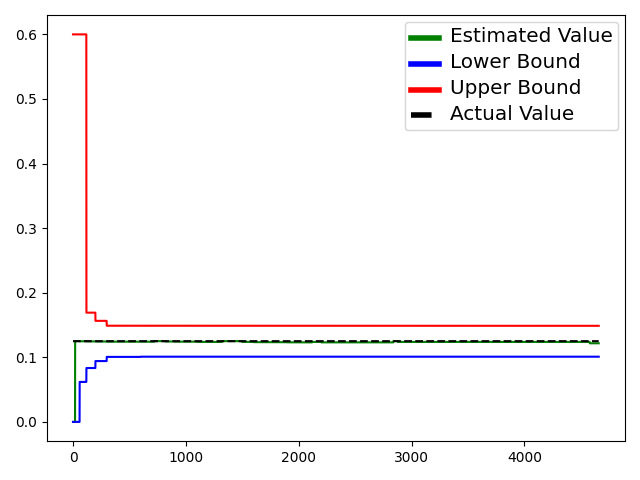
\includegraphics[width=\linewidth]{assets/estim_eccentricity.png}
    \caption{Eccentricity $\mathsf{e}$ of the Orbit}
    \label{fig:results_estim_eccentricity}
  \end{subfigure}
  \hfill
  \begin{subfigure}[b]{0.48\textwidth}
    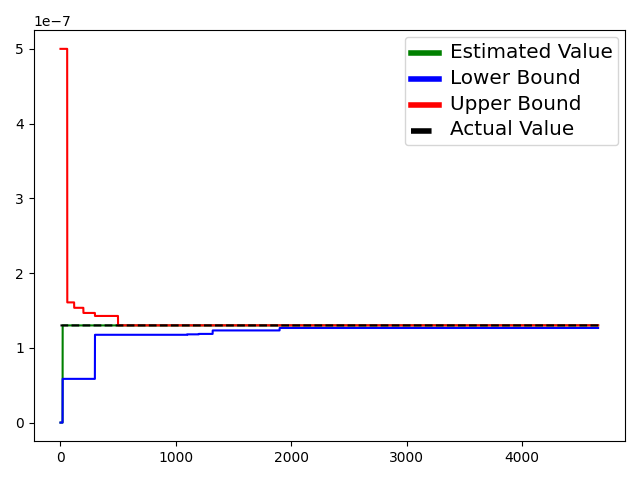
\includegraphics[width=\linewidth]{assets/estim_alpha.png}
    \caption{Estimation of the Drag Constant $\alpha$ of the Target over time}
    \label{fig:results_estim_alpha}
  \end{subfigure}
  \caption{\textbf{Estimation of Unknown Parameters Over Time}}
\end{figure*}

\subsection{Analysis of ADTMPC and other techniques}
\label{sec:results_analysis}
We perform the following analysis to depict the advantages of using ADTMPC over plain MPC.
As is visible from Figure \ref{fig:results_tube}, MPC with and without using adaptive control (and hence the estimation of the unknown parameters) leads to the violation of the chaser-target collision constraints.
% One figure containing four subfigures demonstrates the violation of constraints
\begin{figure*}[b]
  \begin{subfigure}[b]{0.49\textwidth}
    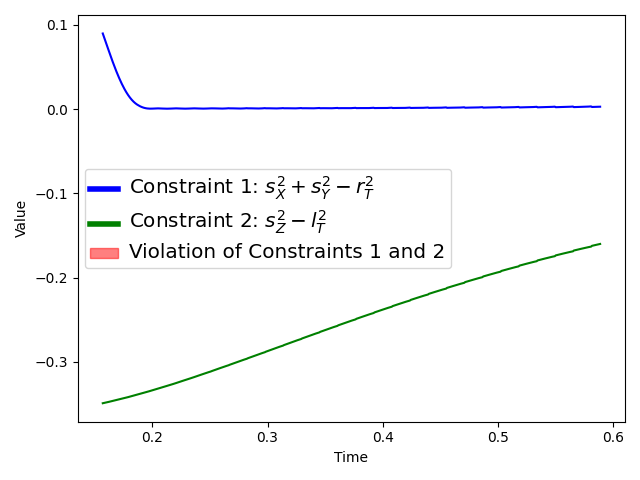
\includegraphics[width=\linewidth]{assets/results_with_tube_dtmpc.png}
    \caption{Dynamic Tube MPC}
    \label{fig:results_with_tube_dtmpc}
  \end{subfigure}
  \hfill
  \begin{subfigure}[b]{0.49\textwidth}
    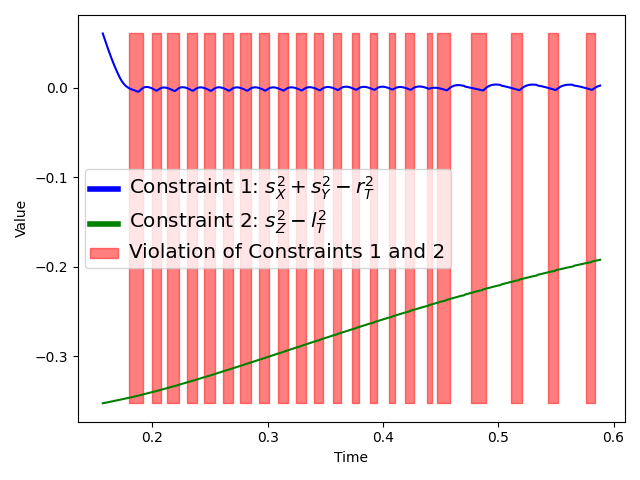
\includegraphics[width=\linewidth]{assets/results_no_tube_mpc.png}
    \caption{MPC (no robust tubes)}
    \label{fig:results_no_tube_mpc}
  \end{subfigure}
  \caption{\textbf{Violation of Collision Constraints without Robust Tubes}: The red regions represent time periods when the collision constraint defined previously as $\boldsymbol{r}(\theta)\in{\mathcal{C}}_D$ is violated.}
  \label{fig:results_tube}
\end{figure*}
Simply using dynamic tubes without adaptation proves to be effective in preventing collisions.
However, due to inaccurate estimates of the unknown parameters and, hence, a large tube, the chaser is unable to converge to the desired docking position on the target.
On the other hand, adaptive dynamic tube MPC shrinks the tube over time, hence allowing the chaser to converge to the final docking position.
Figure \ref{fig:results_adapt} demonstrates how, in very close proximity of the target, previous adaptation of unknown parameters and, hence, a smaller robust tube permits the chaser to move closer to the docking position.
% One figure containing two subfigures one for ADTMPC and the other for DTMPC demonstrates the closeness of the chaser to the target and to the final state.
\begin{figure*}[htb]
  \begin{subfigure}[b]{0.48\textwidth}
    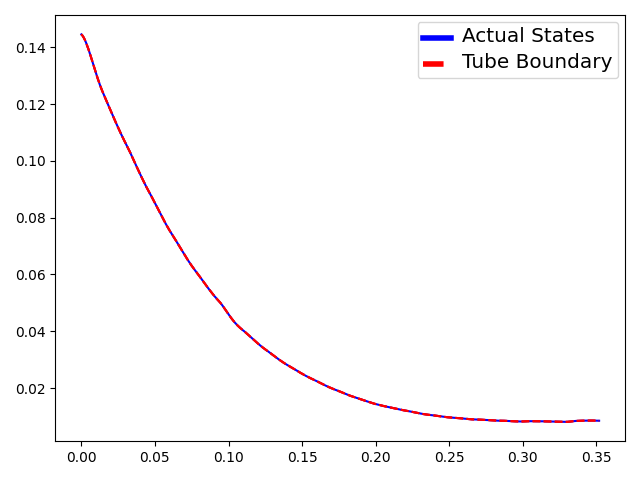
\includegraphics[width=\linewidth]{assets/results_adapt_adtmpc.png}
    \caption{Adaptive Dynamic Tube MPC}
    \label{fig:results_adapt_adtmpc}
  \end{subfigure}
  \hfill
  \begin{subfigure}[b]{0.48\textwidth}
    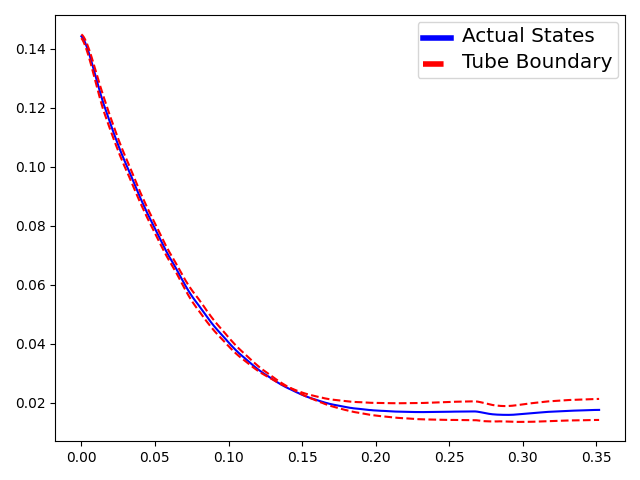
\includegraphics[width=\linewidth]{assets/results_no_adapt_dtmpc.png}
    \caption{Dynamic Tube MPC (no adaptation)}
    \label{fig:results_no_adapt_dtmpc}
  \end{subfigure}
  \caption{\textbf{The Effect of Adaptation}: These plots demonstrate the effect of SMID-based parameter estimation on the size of tubes and, hence, the convergence of the chaser to the final docking point.}
  \label{fig:results_adapt}
\end{figure*}

\subsection{Target Deflection}
\label{sec:results_target_deflect}
Next, we run the optimization problem proposed in Section \ref{sec:target-deflection} such that the chaser attaches to a point within a set of known docking positions and applies a net optimal force to detumble the target.
Figure \ref{fig:results_deflection} demonstrates the results obtained in this regard.
% One figure containing two subfigures one for ADTMPC and the other for DTMPC demonstrates the closeness of the chaser to the target and to the final state.
\begin{figure*}[b]
  \begin{subfigure}[b]{0.22\textwidth}
    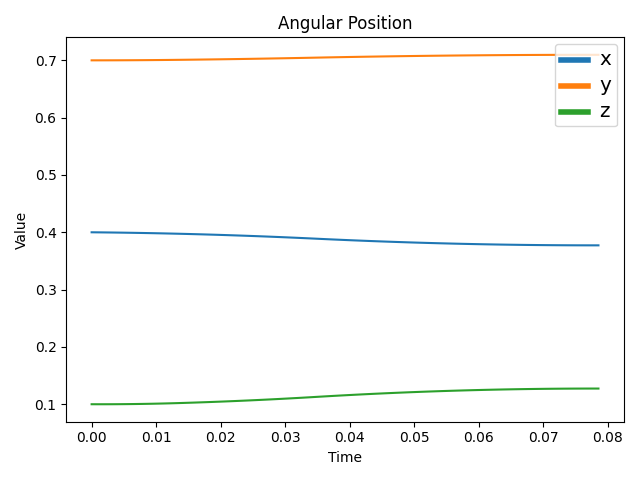
\includegraphics[width=\linewidth]{assets/results_target_angpos.png}
    \caption{Target Angular Position}
    \label{fig:results_target_angpos}
  \end{subfigure}
  \hfill
  \begin{subfigure}[b]{0.22\textwidth}
    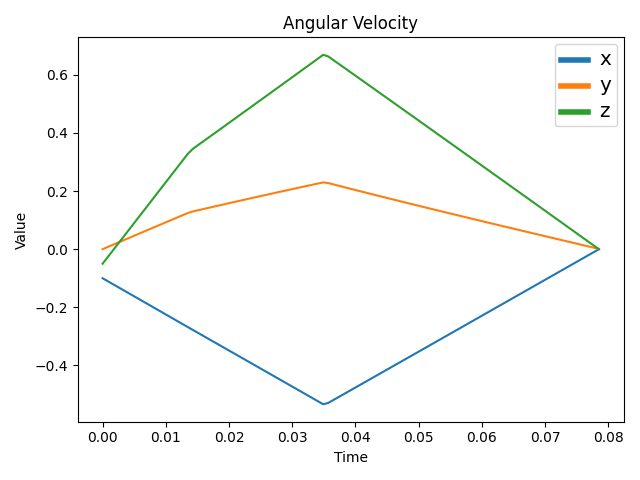
\includegraphics[width=\linewidth]{assets/results_target_angvel.png}
    \caption{Target Angular Velocity}
    \label{fig:results_target_angvel}
  \end{subfigure}
  \hfill
  \begin{subfigure}[b]{0.30\textwidth}
    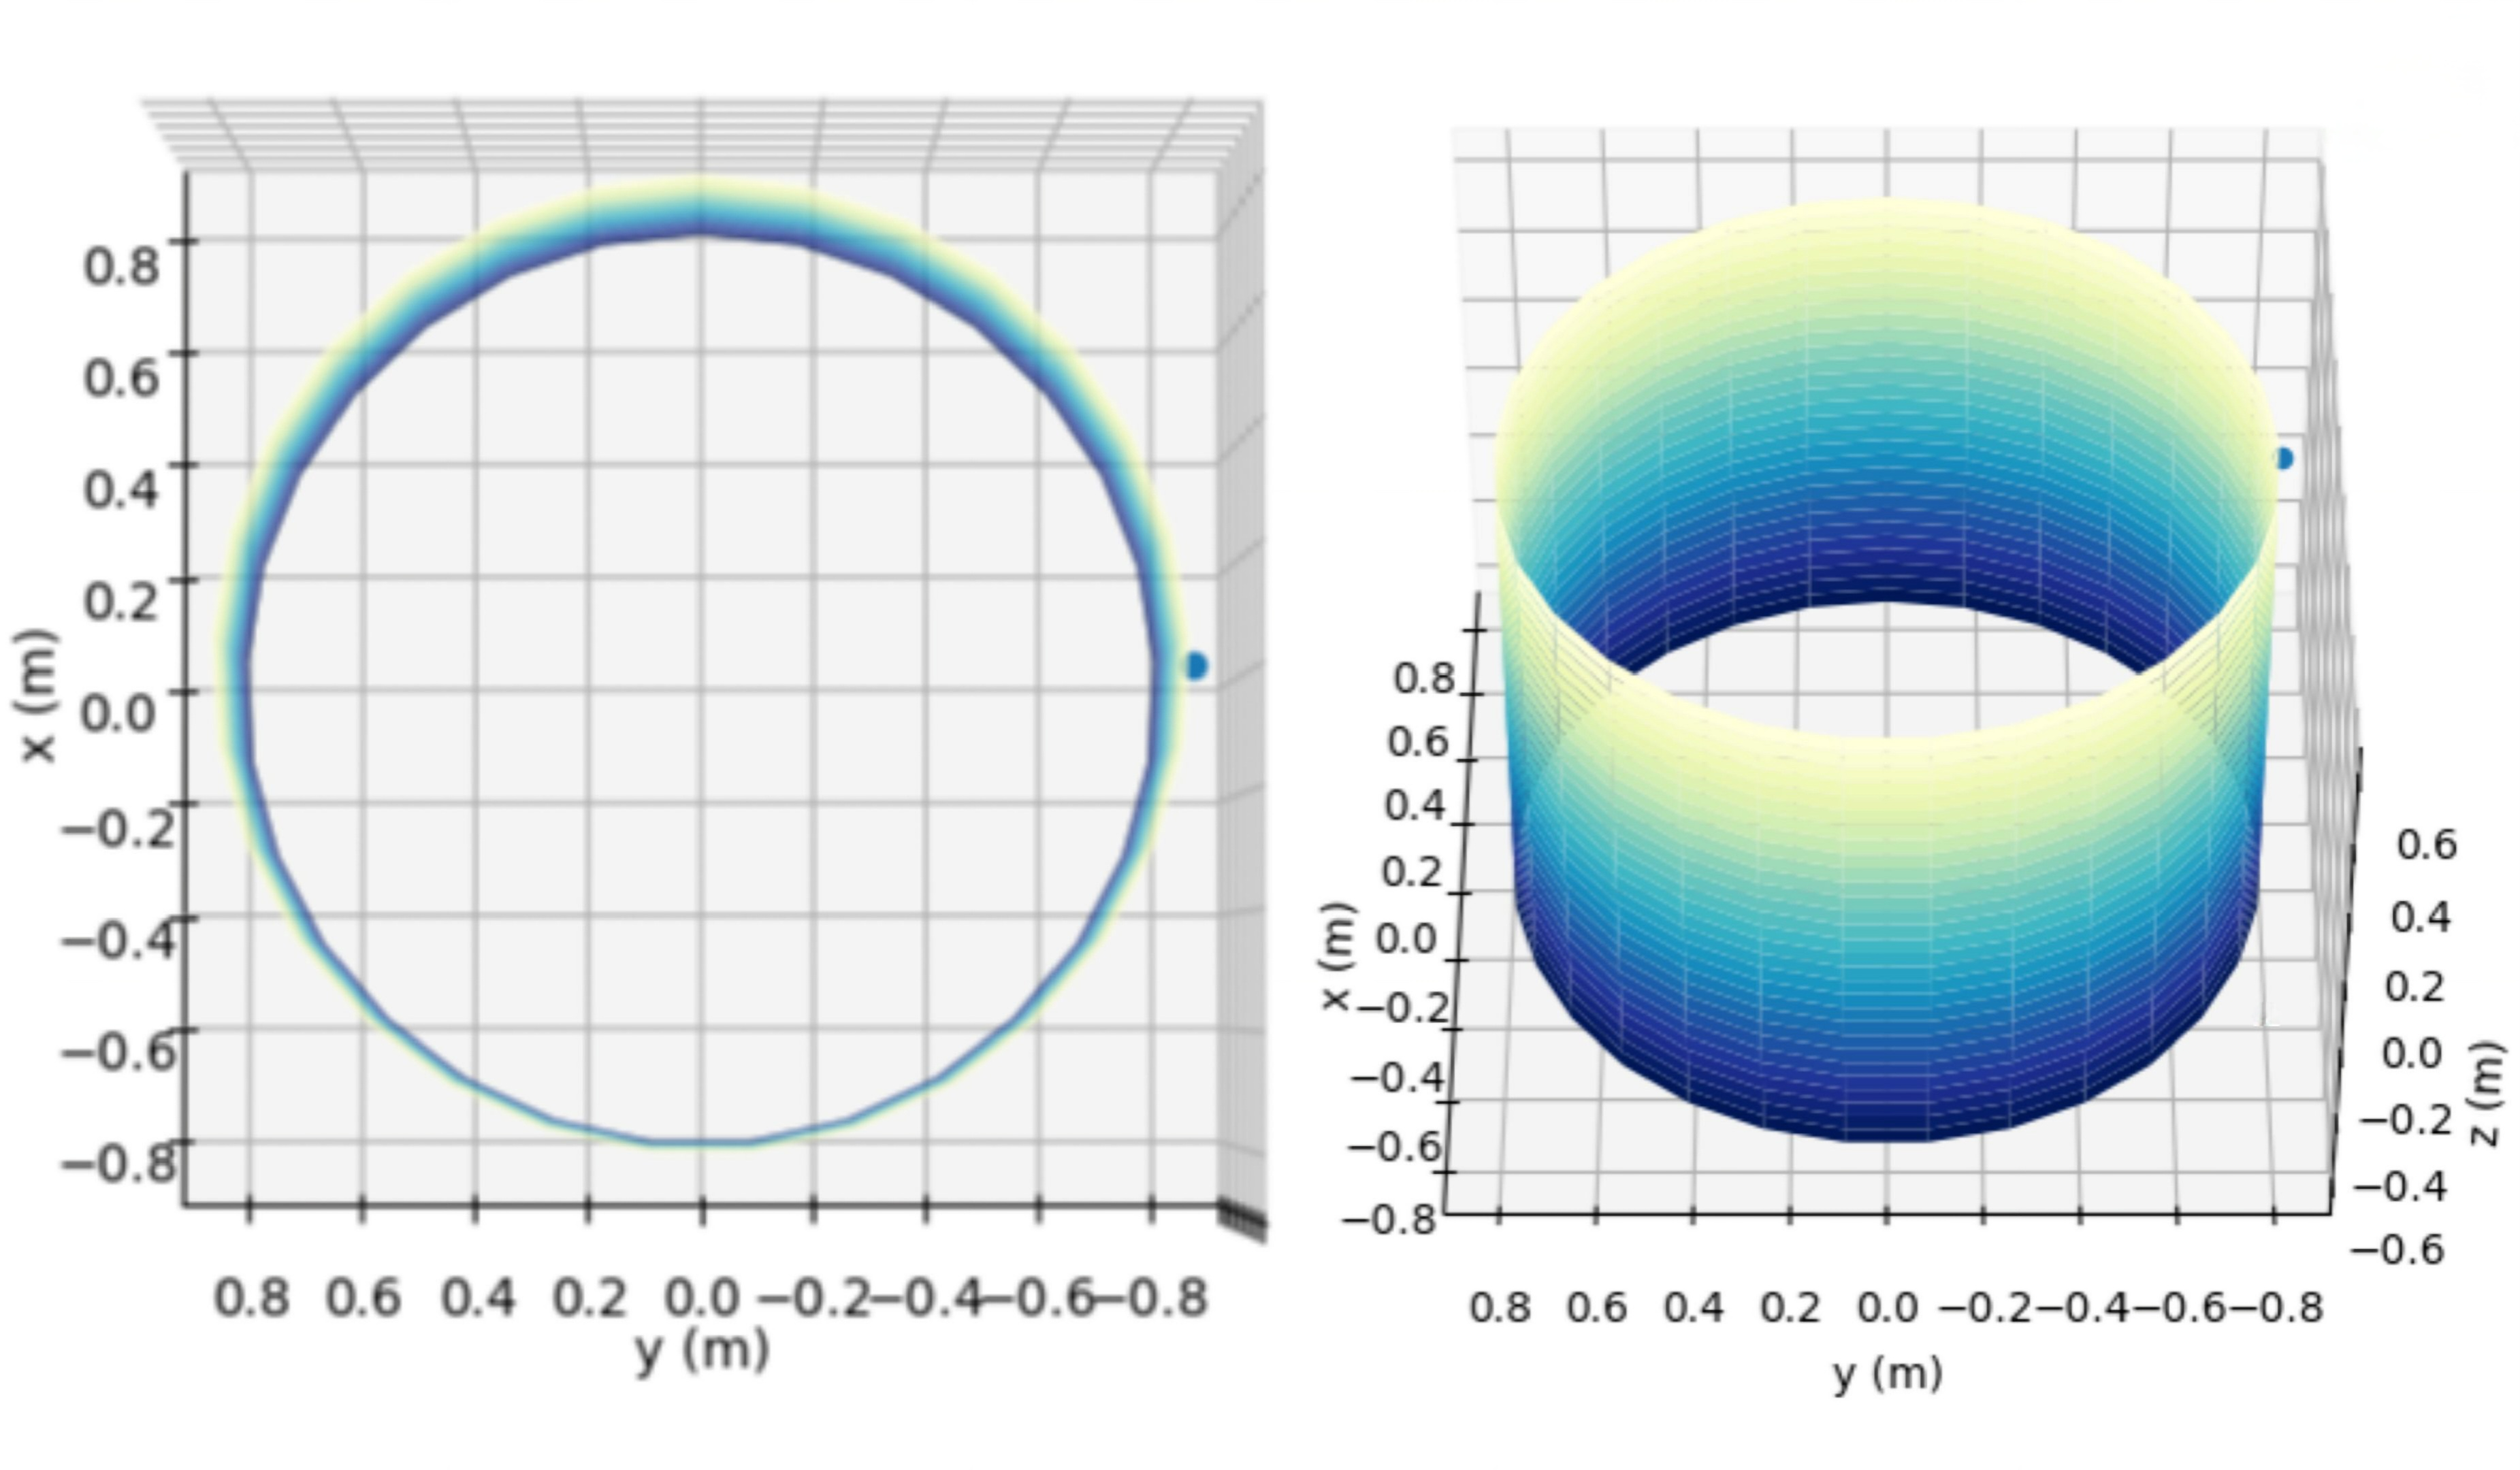
\includegraphics[width=\linewidth]{assets/results_docking_point.jpg}
    \caption{Optimal Chaser Docking Position}
    \label{fig:results_docking_point}
  \end{subfigure}
  \hfill
  \begin{subfigure}[b]{0.22\textwidth}
    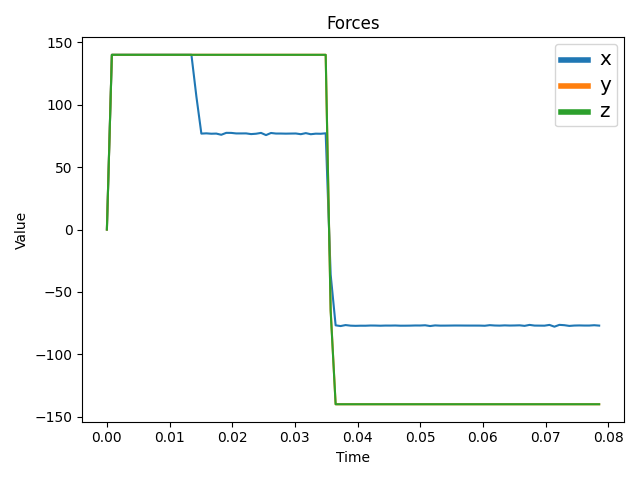
\includegraphics[width=\linewidth]{assets/results_chaser_force.png}
    \caption{Optimal Chaser Force}
    \label{fig:results_chaser_force}
  \end{subfigure}
  \caption{\textbf{Target Deflection}: Subfigures \ref{fig:results_target_angpos} and \ref{fig:results_target_angvel} demonstrate the detumbling of the target such that its angular velocity converges to zero. The blue dot in subfigure \ref{fig:results_docking_point} demonstrates the optimal docking position of the chaser (single-chaser scenario) on the target such that the target is detumbled on the application of force as depicted in subfigure \ref{fig:results_chaser_force}.}
  \label{fig:results_adapt}
\end{figure*}

\iffalse{
\subsection{Observation Spheres}
We do not present results on the implementation of rendezvous and docking using multiple agents.
However, here we demonstrate the calculation of optimal observation spheres given initial and final conditions.
Assuming the target to be a cylinder of radius $r_T=0.6\ u$ and length $l_T=0.8\ u$ (positional units are defined as $u=10\ m$) and the initial ellipsoid to be a sphere of radius $137.5\ u$, the minimum enclosing ellipsoid and hence the final ellipsoid ${\mathcal{E}}_T$ for the optimization problem is defined as:
\begin{align}
    \frac{x^2}{0.980}+\frac{y^2}{0.980}+\frac{z^2}{1.039}=1
\end{align}
We run hyperparameter optimization setting $Q_{\text{local}}=1.0000$ to obtain $Q_{\text{cross}}=0.0960$.
Table \ref{tab:ch5-res-chaser-start} describes the initial positions of the chasers ($N_C=4$).
\begin{table}[h]
    \centering
    \begin{tabular}{|c||r|r|r|}
        \hline
        $i$ & \multicolumn{1}{|c|}{$x_i$} & \multicolumn{1}{|c|}{$y_i$} & \multicolumn{1}{|c|}{$z_i$} \\
        \hline
        1   & $82.392$ & $-47.324$ & $-99.389$ \\
        2   & $80.003$ & $0.0575$ & $111.829$ \\
        3   & $81.752$ & $107.830$ & $24.404$ \\ 
        4   & $43.102$ & $101.807$ & $81.754$ \\
        \hline
    \end{tabular}
    \caption{Result: Chaser Start Positions}
    \label{tab:ch5-res-chaser-start}
\end{table}
On running the optimization problem for $N_L=5$ levels including the initial ellipsoid (${\mathcal{E}}_0$) and the final one (${\mathcal{E}}_T={\mathcal{E}}_{N_L-1}$), we obtain the ellipsoids of the form
\begin{align}
    \frac{x^2}{a_l^2}+\frac{y^2}{b_l^2}+\frac{z^2}{c_l^2}=1,\quad
\end{align}
where the values of the ellipsoidal radii are given in Table \ref{tab:res-optimal-ellipsoids}.
\begin{table}[h]
    \centering
    \begin{tabular}{|c||r|r|r|}
        \hline
        $l$ & \multicolumn{1}{|c|}{$a_l$} & \multicolumn{1}{|c|}{$b_l$} & \multicolumn{1}{|c|}{$c_l$}   \\
        \hline
        0   & $137.500$ & $137.500$ & $137.500$ \\
        1   & $103.315$ & $103.193$ & $103.390$ \\
        2   &  $69.202$ &  $69.012$ &  $69.324$ \\
        3   &  $35.089$ &  $34.914$ &  $35.219$ \\
        4   &   $0.980$ &   $0.980$ &   $1.039$ \\
        \hline
    \end{tabular}
    \caption{Result: Optimal Observation Ellipsoids}
    \label{tab:res-optimal-ellipsoids}
\end{table}
}